\section{Distributed Systems}

    The MARS cloud is architectured as a Distributed system. Thus, it is of great importance to understand
    this architecture, so that one can anticipate how the MARS framework is being operated in the background and
    the technical challenges that could occur due to its complex structure.
    \par
    A distributed system can be defined as a number of autonomous computing elements which 
    appear to a user as a single coherent system. 
    This definition states that a complex system is split into meaningful domains which makes them to behave independent from each other.
    These individual elements mentioned could be either a hardware device or possibly a software process known as nodes. A node can
    be classified from a very high-performance computers with lots of processing power to a simple and cheap computer owned by an average individual. 
    In practice, the nodes must communicate with one another via exchanging messages to achieve certain objective \cite[p.~2]{DistributedSystems}.
    A main characteristics of Distributed Systems is to make the user believe that the system is a single coherent application by supporting 
    resource sharing.

    \begin{figure}[htbp!]
        \centering 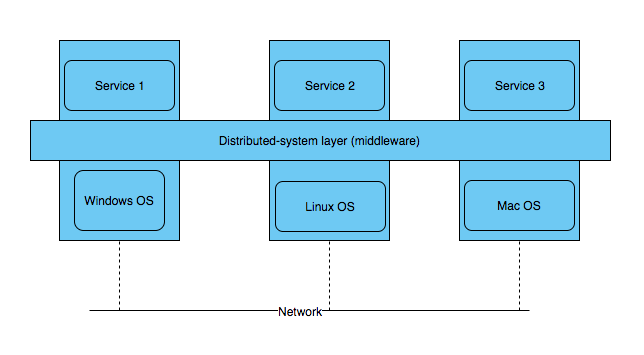
\includegraphics[scale=0.5]{grafiken/distributedSystem.png}
        \caption{A distributed system extended over multiple machine with same application 
        interface \cite[p.~5]{DistributedSystems}}
        \label{fig:distributedSystem}
    \end{figure}

    \newpage
    \par
        Figure \ref{fig:distributedSystem} shows an example of an application being 
        distributed amongst different computers. It can also be seen that the application
        is allowed to communicate via a common middleware whose main responsibility is to
        efficiently manage resources across the distributed applications. This kind of system
        makes most sense for deployment which require high performance computing with fairly
        large number of domains\footnote{domain: A subject area to which the user applies the program in a 
        software \cite{DDD}}.

    \par
        Distributed Systems can be utilized to realize a complex application dispersed across
        multiple machines which communicates via a network protocols(e.g. HTTP \cite{HTTP}, 
        GRPC \cite{grpc}). The 
        components interacts with each other to achieve a common goal. It also provides
        more reliability than a non-distributed system because there is no single point
        of failure when a system is designed properly. 

    \begin{figure}[H]
        \centering 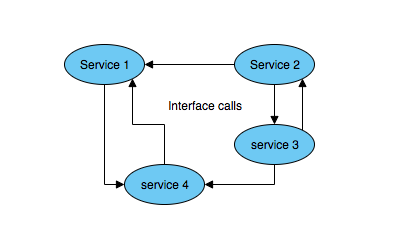
\includegraphics[scale=0.7]{grafiken/objectBasedDS.png}
        \caption{An service oriented architecture in a distributed system 
            \cite[p.~62]{DistributedSystems}}
        \label{fig:objectBasedDS}
    \end{figure}

    \par
        Figure \ref{fig:objectBasedDS} illustrates an example of Service Oriented Architecture 
        (SOA) in a distributed system. The objects/services encapsulates its state and 
        the operations that are performed on the data. This is achieve by exposing an 
        interface to the client/caller to handle any requested operations
        \cite{DistributedSystems}. This architecture allows the objects to be
        completely independent of its environment, thus accomplishing a loosely
        coupled system which is a desired aspect in software engineering.
        
    \subsection{Goals of Distributed Systems} 
        \subsubsection{Reliability and Availability}
        One of the main reasons for building a Distributed system is to make the application free from any single point of failure.
        Since the application is generally spread across different nodes connected via a network, failure of a single node will not 
        crash the program completely. This makes a Distributed system more available, reliable and independent to a user as the availability
        of the application is not hindered completely.
        
        \subsubsection{Scalability}
        Scalability is an important step in software development process, as the requirements for an application tends to changes by time and also requires more resources
        (e.g. more processing power, more data volume). 
        In contrast to a single system, where the computer 
        has to be replaced completely by a really high end device, there is a possibility to just expand the system but adding another device in the network.
        Since the application in a distributed system they are able to communicate via network. Therefore, it is easier to scale and add more resources and 
        also scale down if required. 

        \subsubsection{Increased performance}
        It is desired for a system to have a very good performance metrics which provides the desired results in as short time as possible.
        Distributed Systems provides a possibility to increase the systems performance metrics since more resources can be added to the system,
        the application has more availability of resources it can use. If used properly the application can benefit with an increased performance, 
        which is rather harder to achieve in a single application system. The increased performance comes at the price of its complexity to operate and understand.
        Therefore, it is not very appropriate for a smaller system which can be maintained using a single system.
    
    \subsection{Challenges}    
        \label{subsection: distriChallenges}
        \subsubsection{Data coherency}
        In a Distributed System, it is common for a service or a node to function independently from each other. This brings up the problem that
        one service is not aware of the changes that is done by another. Even though this can be solved by sending messages between the services, the complexity
        level is increased by a great amount when the number of services being used scales up. This is because it becomes cumbersome tasks to communicate with
        multiple services to ensure the right state of the data that is being persisted by the service. This is also mentioned by the CAP theorem, that it is
        impossible to achieve both consistency and availability in the presence of a network partition \cite[p.~59]{CAP}.

        \subsubsection{Network issues}
        Generally in a Distributed System different applications communicate via network protocols i.e. HTTP, GRPC. It is to be noted that
        communication via a network is not always reliable. This is because managing a distributed network is rather complex and due to
        external reasons the communication can break leading to loss of messages which disables some parts of the application. 
        Also, this phenomena would not be seen in a single system.

        \subsubsection{Error Handling}
        Errors are imminent in any kind of application and to continue to work normally again it is necessary to detect and recover from failures.
        Detecting errors in a Distributed System has a different approach since the application is spread across multiple systems and there is no 
        single point of failure. It is not enough that each service ensures its own correctness because the system is interconnected via some kind of
        network connections. Due to the fact that network is also involved in a Distributed System there is additional error detection methods that have
        to be implemented. This brings up more complications in comparison to a single system where an error is contained only in a single system.

         
